\documentclass[blue]{GL2020}
\usepackage{array}
\usepackage{xcolor}
\usepackage{hyperref}
\usepackage{multicol}
\usepackage{ltablex}
\usepackage{tabularx}

\parindent=0pt
\begin{document}
\name{\bWorld{}}

\section*{\pEarth{}}
\pEarth{} is a single continent, divided amongst three nations. The \pFarm{} controls most of the southernmost two thirds of the continent, and the vast majority of the arable land. The \pTech{} dwell in and around the northern mountains of the \pSpine{}. The \pShip{} control a small wedge of land on the eastern coast, and dominate the seas, all the way around the continent and its myriad islands.

Each nation has its own culture, religious customs, and form of government. While the pantheon is shared by all, each nation particularly worships their Patron God. Over \pEarth{}'s long history, the nations have vacillated between cooperation and hostilities. Since on \pEarth{}, murder is forbidden and actively punished by the Gods, much of the tension between nations is played out in ways other than war and bloodshed. A particular sticking point is control of the Storms. These magical Storms manifest once every three years, and will do devastating damage to some portion of the continent, so being able to send the Storm somewhere else is crucial to the advancement of each nation.

No other continents or cultures are known. \emph{(OOC: This is not a game about discovering a new continent or first contact with an alien race or anything like that, and players should focus their game on the situation on \pEarth{}.)}

Here is a \textbf{Map of \pEarth{}} showing the territories of the three nations as well as the College of the Gods. (L’eau is an archaic term for the Wave Riders.)

\begin{center}
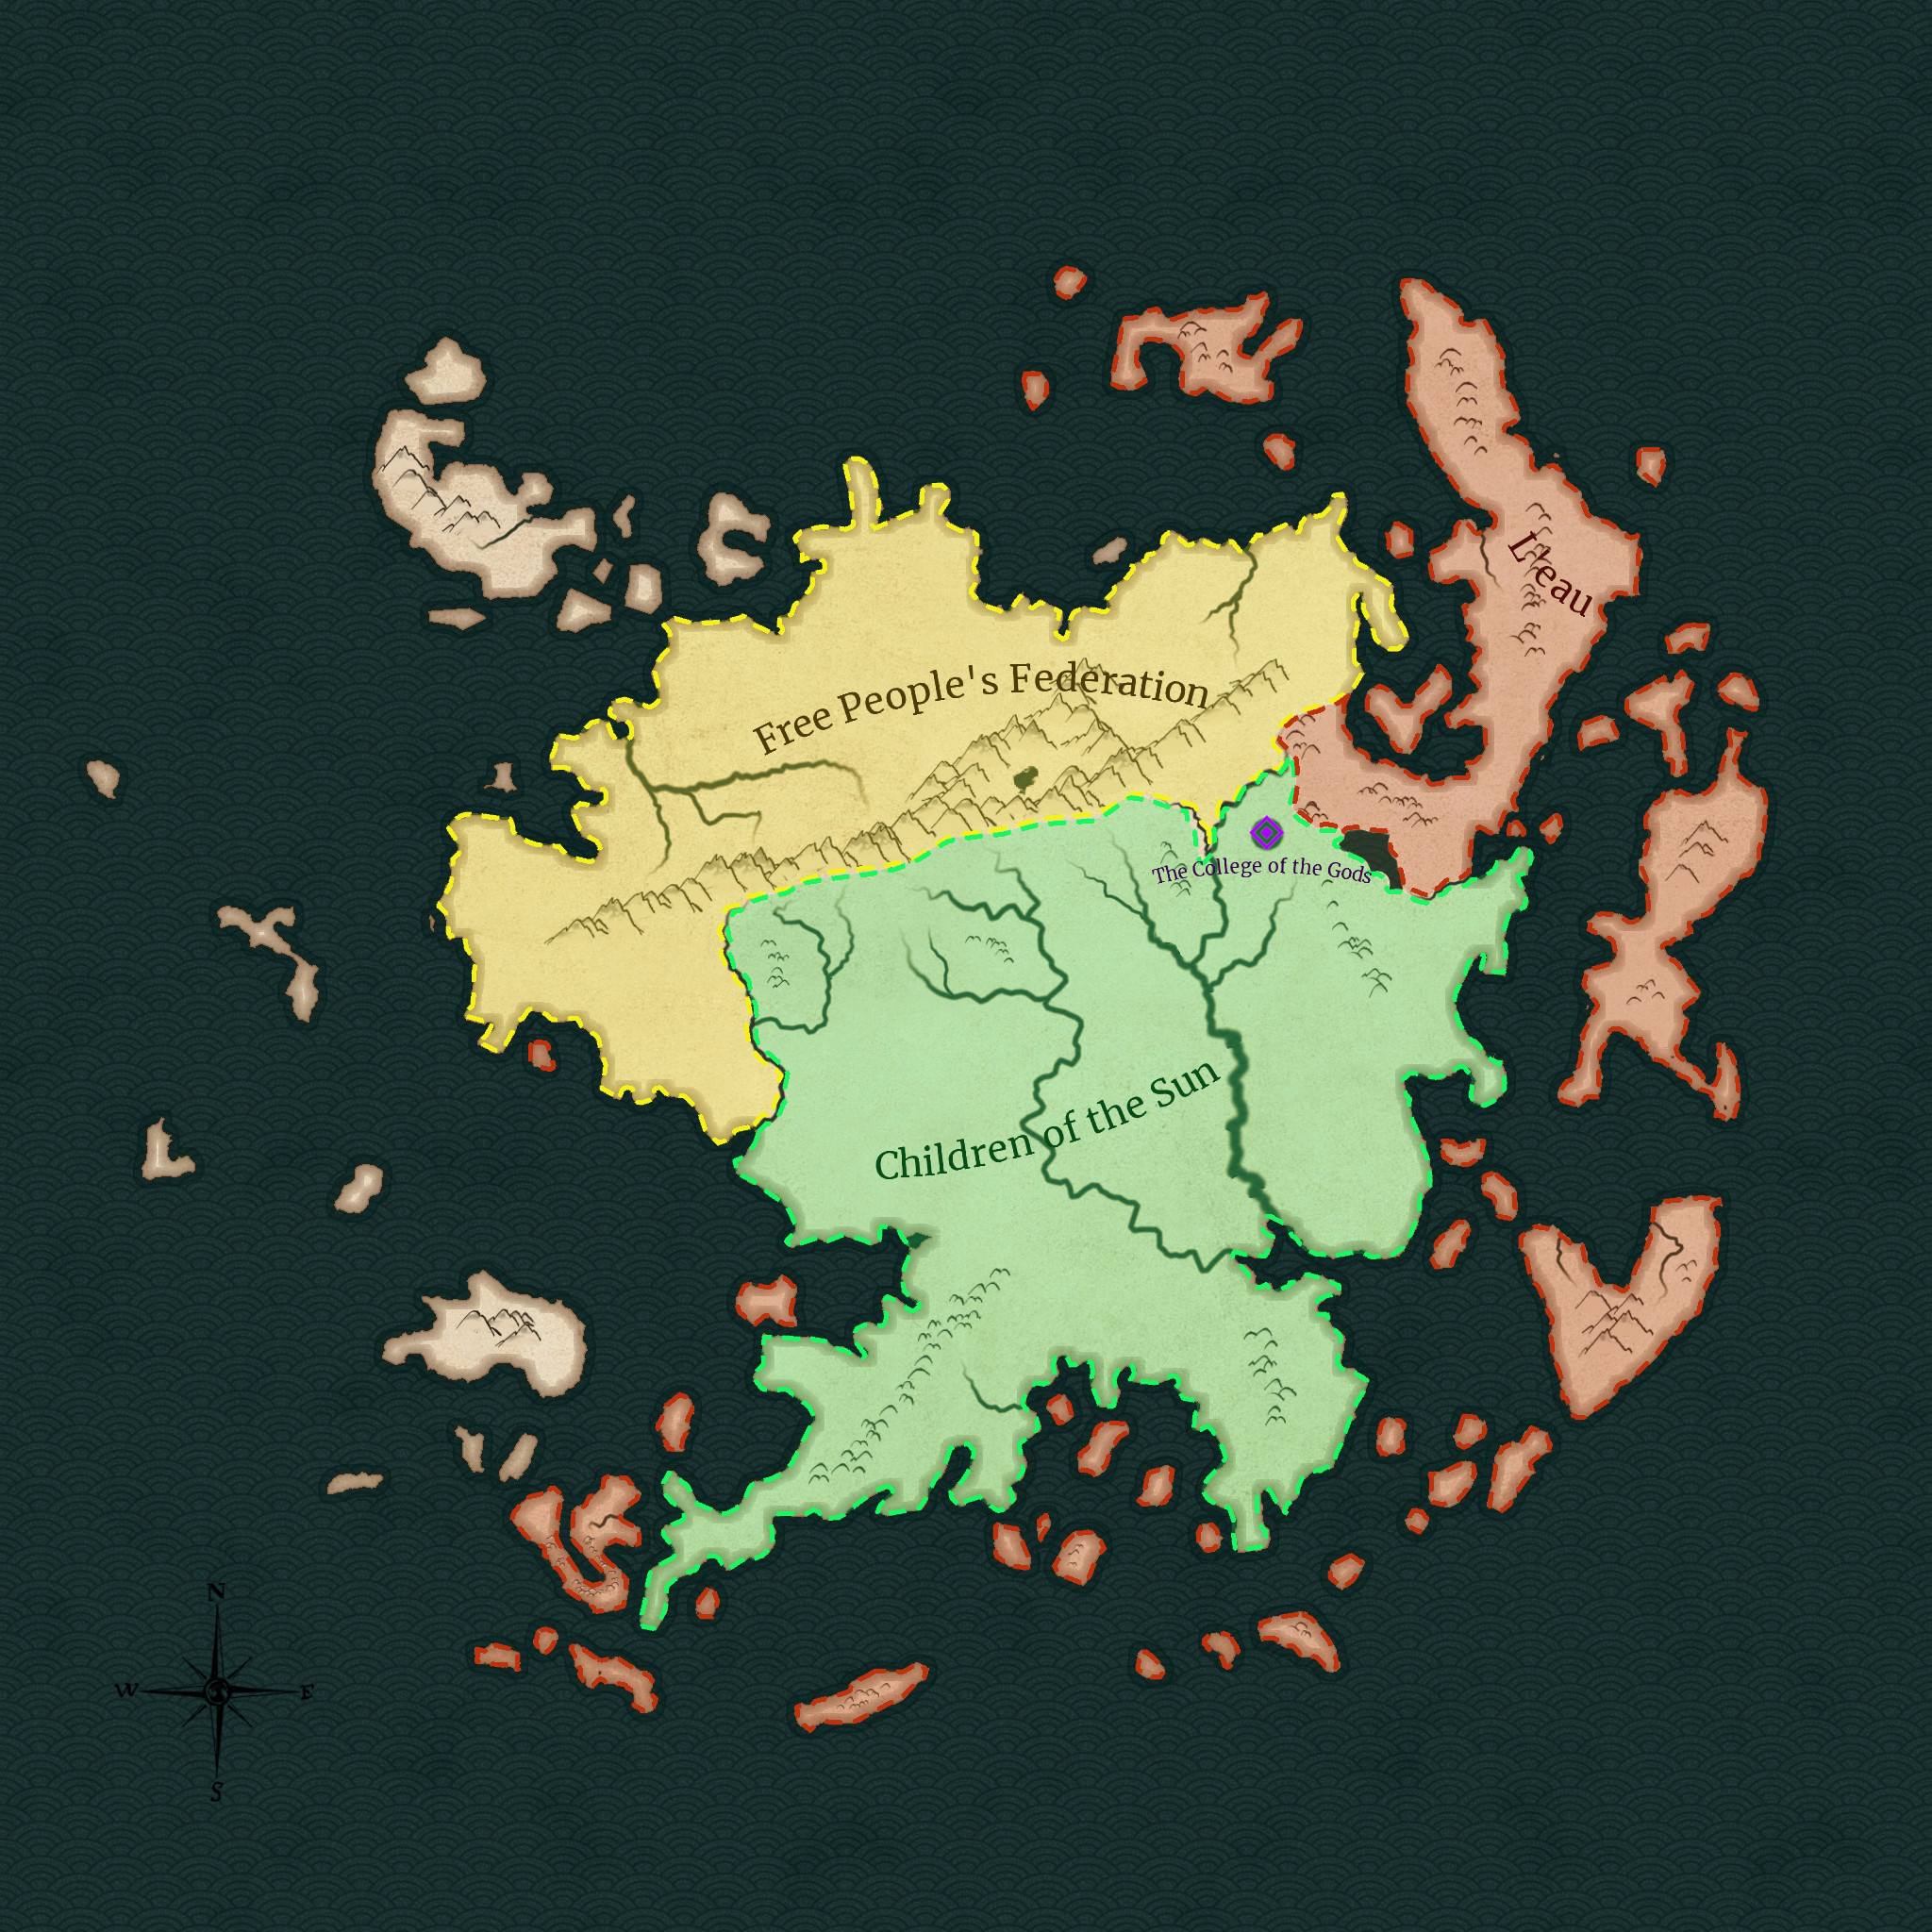
\includegraphics[width=0.6\textwidth]{\gamepath/images/Cengea.jpg}
\end{center}

\section*{Geography of \pEarth{}}

\subsection*{The \pFarm{}}
The \pFarm{} control almost two thirds of the continent to the south, including most of the arable land of \pEarth{}. The climate is Mediterranean, with a long growing season and vast farms stretching as far as the eye can see. The technology level is comparable to the High Middle Ages, with notable exceptions for imported magitech from the \pTech{}. The political structure of the \pFarm{} is a feudalistic monarchy, with most power resting in the hands of the Nobility and the Church. The Nobility works fertility magic that allows the land to grow many times the amount of food it otherwise could, allowing the \pFarmers{} to grow most of the food that all three nations rely on. The common folk work with curses and blessings. The Church controls music magic, which is used for the finest healing in all of \pEarth{}.

\subsection*{The \pTech{}}
The \pTech{} dwell in and around the northern mountain range known as the \pSpine{}. Much of their land is high desert — poor for growing crops, and with wide fluctuations in temperature. Snow blankets large portions of the land, especially in the higher elevations for months of the year. The nation maintains a pretense of democracy and meritocracy, with some government positions subject to popular vote and upward mobility available through higher education, and most citizens believe in this ideal. In actuality, the political structure of the \pTech{} is a more of a theocratic oligarchy, with power shared between the Church and a ruling Council drawn primarily from powerful special interests. The \pTech{} land is rich in mineral resources, especially the gold required for conducting magic, and this has contributed to them being the epicenter of new technology on \pEarth{}. Innovation is prized above almost everything else in the \pTech{}, and as a result, the nation enjoys a level of technology seen nowhere else in \pEarth{}. It has a steampunk flair, but there are no firearms, no engines, and only crude magical batteries. Inventors bring prototypes to the Church for approval. Once approved, the invention can be sent to production and imbued with the magic necessary to make it function indefinitely. Inventors are free to imbue their own prototypes with magic in order to test them, but any attempt to mass produce or distribute them without the approval of the Church is met with swift, divine punishment.

\subsection*{The \pShip{}}
The \pShippies{} of \pShip{} live on their ships, in coastal towns on the continent, in a few settlements on the Eastern floodplain, and on the many small islands surrounding the whole continent. The nation is well into its Age of Sail, dominated by advanced sailing vessels and sophisticated navigational techniques, (but again, no firearms beyond a crossbow). Before the war, the \pShippies{} provided protection from sea serpents to the other two nations, as well as the majority of travel and shipping. Also before the war, the nation's political structure was a consensus based, representative democracy, with a high degree of local autonomy, led by the Council of Storm-Watchers. While this still holds to some degree, with the rise of the Warlord \cLoud{\full} at the start of the war, the nation has begun an alarming slide towards fascism. The magic of the \pShippies{} specializes in craftsmanship of all kinds. The \pShip{} magic is considered the subtlest of all, empowering everything from cooking to shipbuilding , but rarely standing on its own. Only a magical weapon will pierce the hide of a sea serpent. Only a magical sieve can transform seawater to fresh. To leave a debt of any kind unpaid is to disrespect the Patrons \cEbbFull{} and \cFlowFull{}.

\subsection*{The \pSchool{}}
The \pSchool{} sits at the figurative, if not literal, center of \pEarth{}, and is the only truly neutral place on the continent. All three nations send their brightest, best connected, and most magically powerful to the \pSc{}. Most details of the \pSc{}’s founding are lost to time; all that remains in the present is speculation. More information is available in the Magic section below and in the \pSchool{} bluesheet. 

\subsection*{The Oceans and the Sea Serpents}
The continent of Cengea has a fairly large continental shelf, with shallow waters extending a mile out from the coastline. The waters are infested with sea serpents that come in every color of the rainbow. The serpents have always attacked ships and coastal settlements with distressing frequency. No ship that has sailed beyond the continental shelf has ever returned.

The term ``sea serpent'' is unfortunately a bit of a misnomer, as the young live in freshwater, and even the largest have wings that can carry them vast distances. The young are less than a foot long when they are born. They swim upstream from the brackish water in which they hatch, settling in rivers and lakes across the continent, and even stretching their tiny wings to reach terminal lakes. The oldest of the old, past breeding age, leave the water, and fly to the mountain range known as \pSpine{}. They take up residence in caves there, and live out their days ambushing and eating anyone foolish enough to venture into their caves.

\section*{World History}
The planet and the continent (both called \pEarth{}) were created by the Gods — according to ancient religious texts, primarily the four Gods who are now the Patron Gods of each nation. They each then created a people to their own taste, whose descendants still compose each nation (save the odd immigrant who moves from one nation to another, changing their Patron Deity as well). In this way, the people are more than just worshipers — they are the very Children of the Gods.

Even the best kept records in \pEarth{} that go back centuries and centuries do not include a time in which there were more than these three nations, eternally locked in uneasy codependence. Each nation needs things from the others to thrive. But cooperation leaves one vulnerable to betrayal. \pEarth{}'s history is littered with such betrayals, on both personal and national scales.

Still, it seemed like things might have permanently changed for the better after a landmark treaty was signed 34 years ago. Known as the “Time of Peace” treaty, this treaty regulated where the Storm would be sent, allowing each nation forewarning with which to prepare, and ensuring that the burden was shared around equally. According to the treaty, each nation would take its turn to receive the Storm, beginning with the Children of the Sun, then the Free People’s Federation, then the Wave Riders, and then the cycle would repeat every nine years. 

That all changed six years ago, when the \pFarm{} and the \pTech{} forged a new alliance and betrayed the \pShippies{}, sending the Storm to that nation out of turn, when it should have gone to the \pTech{} that year. Immediately following the Betrayal, all twelve students who had performed the ritual to send the Storm to the \pShippies{} were found dead with no sign of external injuries. While the official cause of death was never released, rumors abound that they were murdered. If that wasn't suspicious enough, subsequent investigation revealed that the vote was apparently unanimous. 

The new alliance between the \pFarm{} and the \pTech{} was dubbed "The End of Suffering" by its two member nations. The publicly stated reason for this alliance was that the \pTech{} was on the verge of discovering a means of ending the Storms permanently, and all their progress would be lost if the Storm were to strike them before the project was complete. This promised end to the Storms has yet to materialize, however. Three years ago, in keeping with the alliance, the Storm was once again sent to the \pShippies{}, devastating this seafaring nation that had not yet fully recovered from the previous Storm.

\subsection*{The War}
Ever since the Betrayal, the \pShippies{} have been at war with the other two nations. War in a world where murder is forbidden by the Gods is a strange thing. Since it is impossible to field armies (attempts have been made historically; they all ended in mass confusion quite quickly), the war is waged indirectly. The \pShippies{} drive sea serpents onto the shore, where the creatures wreak havoc before escaping back into the ocean. The \pShippies{} have caused significant damage to settlements in proximity to bodies of water in both other countries this way, and have staked claim over many coastal and riverside areas around the continent as a result.

For the first few years of the war, the \pFarm{} and the \pTech{} had little answer to the \pShippies{}’ raids. But after much bloodshed, they finally developed the technology to use massive trebuchets from the \pTech{} to launch curses from the \pFarm{} at \pShippie{} ships. The trebuchets are massive undertakings to build (especially without the craftsmanship of the \pShip{} magic users), and must be built as permanent installations. There are a few grand and far off plans of mobile trebuchets that could be used for an offensive, but for now, they are primarily useful as defensive installations.

In turn, the \pShip{} are innovating as well. They are starting to send landing parties with the sea serpents, cutting off their retreat and driving the serpents further inland than they would otherwise go. This tactic is too new to know whether it will have a significant impact on the war.

\section*{Religion}
Religion is a deeply important part of the cultures on \pEarth{}, and in individual lives. Everyone knows at least one person who has spoken to the Gods in a dream, or through one of their Avatars. Many people have had prayers answered through obviously divine intervention. Those who do not take religion seriously are shunned, and so those few who feel less drawn to, or less supported by the system, tend to keep that to themselves and pretend in public.

\pEarth{} has a large pantheon of Gods, but the most important are the Patron Gods:
\begin{itemize}
    \item \cFarmGod{}, \cFarmGod{\God} of the sun, music, and the living world, Patron of the \pFarm{}.
    \item \cTechGod{}, \cTechGod{\God} of ingenuity, science, and engineering, Patron of the \pTech{}.
    \item \cEbbFull{\full}, reigns over the sea, ships, and things lost or taken, who along with \cEbb{\their} twin \cFlowFull{} is Patron of the \pShip{}.
    \item \cFlowFull{\full}, reigns over the sea, the rain, and things created or given, who along with \cFlow{\their} twin \cEbbFull{} is Patron of the \pShip{}.
\end{itemize}

Further details about each Patron God can be found in their corresponding nation's bluesheet. \pEarth{} can be said to have a single world religion, but its interpretation and application vary fairly widely between the nations. Clerics of all four deities are treated with respect, and in turn offer council and sanctuary to all, regardless of their patron. Each nation primarily worships their Patron, but will offer small gestures to the others, even in their homeland, especially when asking a boon that falls under another God's purview. When visiting another nation, it is considered a huge faux pas to not engage with their religious services and traditions. When the situation warrants, most people also pay homage to the countless Minor Deities of the pantheon (more details to be released later in the Pantheon bluesheet).

Almost every single citizen of a given nation is a devotee of that nation’s Patron Deity. Likewise, almost every single devotee of a given Patron Deity is a citizen of the nation that claims that Patron. In each nation, there are no clerics of the other deities to tend to any such devotees; they would be completely isolated from their practice. Vice versa, no cleric practices in a nation not of their Patron Deity, as they lack the necessary support structure, and have no devotees to support. Ultimately these truths all feed on each other, making it impractical at best and impossible at worst to live in a given nation and not have that nation’s Patron Deity as your own Patron. On those rare occasions in which someone immigrates, foregoing one’s former Patron is an expected part of the process.

While many Gods exist, the Patron Gods set the rules of \pEarth{}, granting power to those who follow their teachings, and punishing those who disrespect them. The Patrons are matched in power, so each individual need only follow the teachings of their Patron God. Minor Gods can grant small blessings when invoked properly, but lack the authority to issue punishment, or the power to protect worshipers from the Patron Gods.

\subsection*{The Creation Story}
In the beginning, all of the Deities were equal in the nothingness. \cFarmGod{}, \cTechGod{}, and the twins \cEbb{} and \cFlow{} got together and decided, in their infinite wisdom, that what was needed was a world. And so they went to the other Gods, and through persuasion, logic, trickery, bribery, and unexpected kindnesses, convinced the entire pantheon that they were correct. And so the Deities brought their power together and created \pEarth{}. Upon it they placed the single continent by the same name. This single land mass represents the cooperation of all the Gods, and the wonders that they could create when united. When the primary work was done, a council was called among all the Gods to determine who would create the race of beings most like the Deities themselves. The vote was unanimous. Those who had originally brought the idea should create its crowning glory. And so \cFarmGod{}, \cTechGod{}, and the twins \cEbb{} and \cFlow{} set about creating humanity, each in their own way. The four Deities then pooled much of their remaining power together for a gift for their new Children — the gift of magic. This gift would help them weather the Magical Storms that ravaged \pEarth{} every three years.

\subsection*{Clerics of the Gods}
Clerics are the keepers of religious lore and tradition. They lead ceremonies, provide counsel to individuals, and guidance to governments. As all magic comes from the Gods, they are also often the primary keepers of magic in a community. While people generally prefer to go to Clerics from their own nation, any Cleric should be able to provide sound, non-partisan advice to a person in need.

\subsection*{The Avatars}
Each Patron Deity has one or more Avatars on \pEarth{}. These beings are conduits of the Gods' power, and each takes the form of an animal. \cFarmGod{}'s Avatars are giant hummingbirds the size of small wagons. \cTechGod{}'s Avatars are scarab beetles known as the Celestial Beetles for the iridescence of their shells is more enchanting than the night sky. And \cEbb{}'s and \cFlow{}'s Avatars are two sea serpents of immeasurable beauty — one with silver scales, and the other gold. These Avatars will often serve as the mouthpieces for the Gods, bearing messages to Clerics and chosen heroes. The Avatars are also a source of power and connection. Magic too difficult to do any other way can be done in the presence of an Avatar. If an Avatar were to be lost, it would severely hinder the Deity's ability to impact life on \pEarth{}.

\subsection*{Morality and Murder}
Each Deity, and therefore each nation, has their own views on morality, with one exception: taking of another human's life. Committing murder will earn you immediate and complete amnesia, the punishment handed down directly by the Gods.

Social opinions on those who have been struck with amnesia are split. Most people ostracize amnesiacs, unwilling to trust someone who has killed, even after all their memories have been purged. Shunned by society and bereft of their memories and former social ties, most amnesiacs thus face a grim and lonely fate. A small minority of people see amnesiacs as unfortunates who now have the possibility to become better people. The circumstances that drive someone to kill are seen by these few as a matter of nurture rather than nature. The most fortunate amnesiacs are able to find small enclaves of such individuals, where they are accepted, reintegrated into society, and given the support they need to build new lives.

\subsection*{Rejecting the Gods}
To be an atheist in Cengea is almost unthinkable. Even setting the vast societal pressures aside, claiming a patron Deity protects you from the rules of the others. Therefore, an atheist, far from being free from the Gods, is subject to 3 sets of rules and taboos rather than just 1, as well as the threat of displeasure from the divine with no recourse. An atheist is also denied the Gods' gift to their children — the ability to use magic. It is a difficult and thankless lifestyle, chosen only by the most defiant or resolute. No characters in game are publicly atheists.

\subsection*{Magic}
Magic has been a part of \pEarth{} since essentially the beginning. It is said that the Patron Gods themselves granted humanity magic, breathing life into the Ley Lines, as a gift to help them survive the Storms that have raged across the world every three years since time immemorial. The three nations then took that gift and perfected it, building the \pSchool{} on top of the floating island where the Ley Line Nexus is located. At this focal point of power, ancient mages developed the Ritual to Control the Storm (see next section).

While there are many things in the world of \pEarth{} that an outsider might consider magical, the term ``magic'’ is reserved for the power that humans wield, and the things they create with it. Almost every aspect of life in all three nations is dependent on magic in some way, from the fertility magic in the \pFarm{} that makes the crops grow bountiful, to the magitech wonders of the \pTech{} that enable that nation's industrial age, to the crafting magics of the \pShippies{} that keep their ships seaworthy and their fishing gear from tangling.

Magical ability manifests at a young age, usually beginning to show at around 5 or 6. While it's hard to measure the raw potential of a completely untrained magic user, it is generally believed that the younger the user, the more raw power they wield. Of course, magic is nothing without control — so the strongest magic users are young geniuses who learn to wield their power at a young age. For the purposes of the Ritual to Control the Storm, college age is considered the ideal balance between power levels and magical knowledge. This is not to say that elders in \pEarth{} who were magical in their youth are without magic now. They still have power, but it is more specialized and limited in scope. They must use skill and cleverness to address problems they might previously have been able to solve with brute force.

Magical potential resides inside people, usually with little concept of exhausting one's store. (OOC: Your character's Combat Rating [CR] represents a combination of their inherent magical reserves and their knowledge of how to wield them in combat.) The exception involves a special class of items called \textbf{Tass}. Tass items are able to store magical energy outside of a person for use later. Tass is very difficult to create, taking months to fabricate an item capable of holding a single unit of magical energy. Once the Tass is created, however, any individual may voluntarily deposit some of their magical energy into it. (OOC: This will cause a temporary reduction in your CR — the Tass item will have more details.) Only a select few individuals know how to extract the magical energy from the Tass and make use of it.

\subsection*{The Storm}
Every \pCycle{} years, a Storm brews on the lake below the \pSc{}, cutting off access to the island for several days at the halfway point between the fall equinox and the winter solstice. No one knows what causes the Storms, but theories abound, from a punishment from the Gods for the collective sins of humanity now lost to history, to the cruel depredations of evil spirits, to a simple natural phenomenon. Regardless of the reason, the Storm waxes and wanes in power as it builds. After building in power for several days, the Storm spins off to wreak havoc across all of \pEarth{}. This catastrophe can be partially averted by twelve hand-picked Students at \pSchool{} enacting the Ritual to Control the Storm, directing its wrath towards one of three areas: The \pFarm{}, the \pTech{}, or the coastlines and outlying islands where the \pShippies{} live and work. 

While devastating to whichever nation the Storm was sent to, the total damage is far less than what is wrought across the entire continent by an uncontrolled Storm. Every effort in the past to mitigate the damage done by the Storm has failed. No matter how people try to avoid the harm, whether by sending the Storm to a remote location or evacuating the area, the same failure occurs — the Storm escapes control of the Students and wreaks havoc over the entire continent before dissipating. In the end, more damage is done to all three countries than would have been done to a single nation if the attempt had not been made. Eventually people gave up trying to outsmart the Storm somehow.

\section*{The Time of Deciding}
This weekend is the ``Time of Deciding.'' This weekend the Storm is brewing under and around the \pSchool{}, and must be sent somewhere. The people at the school are the ones tasked with this decision. \textbf{Assuming the Ritual to Control the Storm is completed, three factors influence where the Storm will go: A vote held by the Students using the Voting Stones (this is the largest factor), which nation(s) the Relics used in the Ritual to Control the Storm are attuned to, and where any treaty signed by the Advisors and ratified by at least two nations’ governments says the Storm should go.} 

\subsection*{Voting Authority}
Four Students from each nation are selected to stay at the \pSc{} during the Time of Deciding. They must take on the massive responsibility of performing the primary role in the Ritual to Control the Storm. Students are selected based on their magical power and academic performance relative to their peers. It is one of the highest honors a Student can receive, and it can have a lot of influence on their future after they graduate. Joining the twelve students are twelve Teachers and twelve Advisors, four from each nation in each cohort. Presiding over the entire affair is the immortal Principal of the \pSchool{}.

Each Student, Teacher, and Advisor present at the Time of Deciding receives one Voting Stone. Teachers and Advisors must select which Student to give their Voting Stone to, as only Students can cast votes. Once given to a Student, the stones magically bind to the recipient and cannot be transferred to anyone else. Each student can hold up to 5 stones maximum. If someone tries to give them a sixth, the transfer does not work. When it comes time to vote on where to send the Storm, each Voting Stone held by a Student counts as one vote. As such, each Student may cast anywhere from one to five votes for where to send the Storm, depending on how many Teachers and Advisors they have won over and received Voting Stones from.

\subsection*{Influencing the Voting}
During the Time of Deciding, Advisors from each nation come to the school to guide and influence the Students. Since the Students are young adults, it is crucial that the Advisors explain the consequences of the various options, given the current political landscape. The Teachers are ostensibly neutral parties in the discussion, but few have no opinion on where the Storm should go, and Students often take counsel from Teachers as well. Since the Advisors have no direct control over the student vote, they take the task of influencing the Students quite seriously. Different Advisors will employ different tactics to try to influence the Students, but outright threats are generally frowned upon. At the very least, each Advisor can offer the enticement of an internship to a student who votes their way, as well as the Voting Stone they begin the weekend with. Teachers have Voting Stones to dole out as well, and thus have some of their own leverage, despite their supposed neutrality.

\subsection*{Storm Surges and The Bunkers}
During the Time of Deciding, the Storm is brewing. Three times over the course of the weekend, the Storm will surge in power, and it will become dangerous to be out and about at the \pSc{}. There are three Bunkers installed at the school which provide protection from the physical, mental, and magical damage that the Surges can do to an unprotected person.

\subsection*{Voting to Control the Storm}
Beginning Sunday morning, Students will be able to cast their votes for where to send the Storm. Students are strongly advised to have a good idea of how they want to vote \emph{before} Sunday morning, as any votes not submitted by 11:30 am are forfeit.

\subsection*{The Ritual to Control the Storm}
Over the course of the weekend, the Ritual to Control the Storm must also be prepared. Several Teachers are well versed in the preparations necessary, especially \cLibrarian{\full}, and will be leading the effort to organize the Relics and other preparations. The Students have an important role to play in preparing for the ritual as well (if you are a Student, see the Student bluesheet). On Sunday afternoon, the ritual will be enacted, requiring the participation of almost everyone at the \pSchool{}. If the Ritual to Control the Storm is not completed, the Storm will rage unchecked across all of \pEarth{} as it did in the days before the \pSchool{} existed, which would be an unmitigated catastrophe.

\subsubsection*{The Relics}
The Relics are objects of incredible magical power. Some are gifts from the Gods and others were forged by particular groups of humans, as epic and heroic feats. Regardless of their origin, the Relics are handed down as national heirlooms. The Relics are either stored in the \pSchool{} Library permanently, or brought to the \pSc{}during the Time of Deciding. The Relics can work miracles when they are attuned. Attuning a Relic can only be accomplished by trained clerics near the fully charged Ley Lines that run beneath the school during the Time of Deciding. Attuning a Relic both powers it up and focuses its protective energies on one of the three nations. In the Ritual to Control the Storm, each Relic used that is attuned to a given nation reduces the odds that the Storm will be sent to that nation. Two common arrangements are to either have all three Relics used in the Ritual attuned to one nation, indicating the Teachers’ opinion of which nation the storm should \textbf{not} be sent to, or to have one Relic attuned to each nation, suggesting a more neutral stance. Any combination of attunements is acceptable, as long as all three Relics are attuned to \textbf{somewhere}. Using a Relic for the Ritual to Control the Storm, or using its other miraculous properties, deattunes the Relic. Choosing which of their Relics to use in the ritual and which to save for other purposes is an important decision facing each nation.

\begin{tabularx}{\textwidth}{|>{\centering\arraybackslash}c | >{\centering\arraybackslash}c | >{\centering\arraybackslash}c | >{\centering\arraybackslash}c |}
\hline
    \multicolumn{4}{|c|}{\textbf{The Relics}} \\
\hline
    \emph{\textbf{Relic (item number)}} & \emph{\textbf{Associated Nation}} & \emph{\textbf{Usual Location}} & \emph{\textbf{Known Powers}}\\
\hline
    \iPitcher{} & \pFarm{} & Advisor Delegation & Powerful healing\\
\hline
    \iScythe{} & \pFarm{} & Library & Powerful weapon\\
\hline
    \iMirror{} & \pTech{} & Advisor Delegation & Long distance scrying\\
\hline
    \iLariat{} & \pTech{} & Library & Compels honesty\\
\hline
    \iChalice{} & \pShip{} & Advisor Delegation & Purification, removes afflictions\\
\hline
    \iNet{} & \pShip{} & Library & Can catch anything, controls the tides\\
\hline
\end{tabularx}

Other Relics have existed throughout history, but have been lost or destroyed. In theory, the knowledge still exists to create a new Relic, but it is a truly legendary undertaking.

\subsection*{A New Treaty?}
When the Time of Peace treaty was broken 6 years ago, and the \pShip{} was struck out of turn, the tenuous peace was shattered. Still, after so many years of war, more and more people are willing to consider a new peace treaty, or at least a ceasefire of some kind. Opinions are deeply divided on whose turn it would be to take the Storm's fury, however, if such a treaty were to be signed. Any attempt to reforge the treaty will be a fraught affair and successful adoption will require ratification by home governments (managed by the GMs), all of whom are likely to be picky and stubborn about the terms. What's more, any new treaty signed and ratified by at least two nations’ governments will carry metaphysical weight — any stipulation in the treaty regarding where the Storm should be sent will influence the actual destination of the Storm at this Time of Deciding.

\end{document}

